
\chapter{Introduction} \label{chapter:introduction}
\section{Overview} \label{section:introduction:overview}

Many robotic applications, especially those that involve human-robot
interaction, often require a rich representation of the environment in order to
perform such behavior as path planning and obstacle avoidance. In general, a
rich representation, or map, is useful for providing situational awareness to an
autonomous agent. A map is also important for applications such as teleoperation
\cite{Kadous2006}.

The methodology to build this representation is a continuously evolving subject
in the field of robotics. The origins of the research into this problem date
back roughly 25 years \cite{Lorensen1987}. Since then the methods and the
representations themselves have continued to evolve at an impressive rate. The
main catalyst behind this growth is the advancement of sensing technologies over
the same time period. In general, sensors have continued to generate
measurements at higher rates, higher resolution, and lower cost over the years.
This has provided an amazing opportunity to build richer and more useful
representations of the environment.

In robotics, map building in an unknown environment is referred to as the
Simultaneous Localization and Mapping (SLAM) problem \cite{Thrun2002}. This
label describes the fact that a methodology which solves the SLAM problem must
simultaneously locate the robot in the environment as well as map the
environment. The focus of this work is the mapping aspect of the SLAM problem.
Fig. \ref{fig:goal} gives a visualization of the goal.

\begin{figure}[h]%[thpb]
\centering
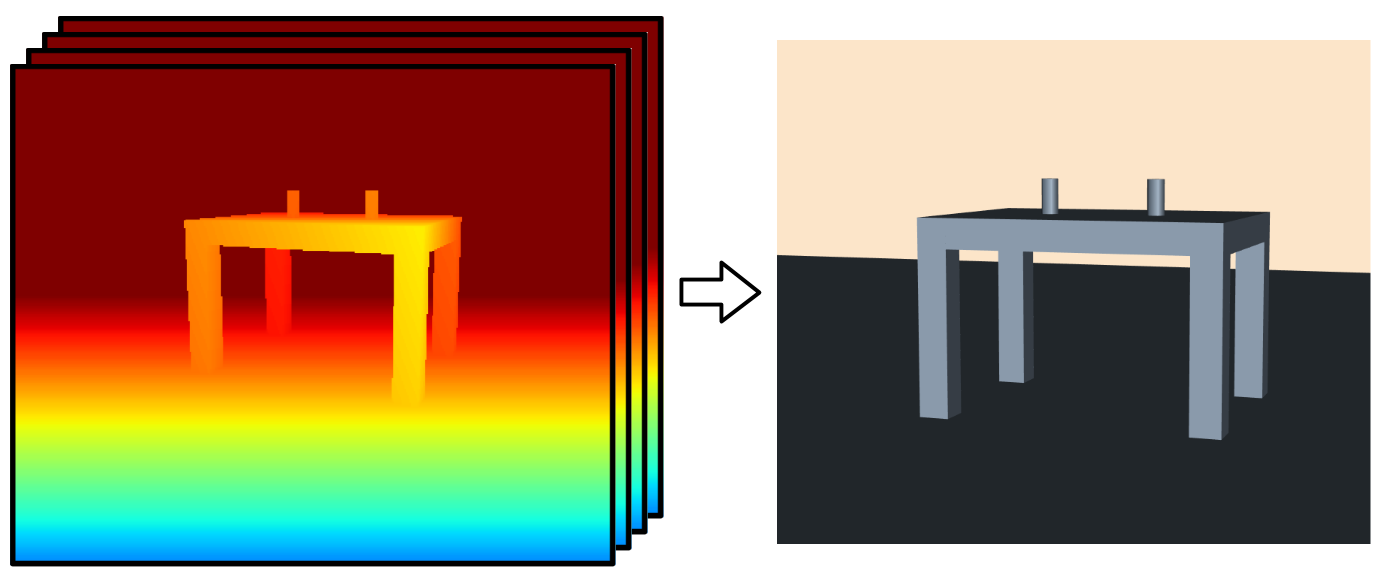
\includegraphics[width=.75\textwidth]{figures/diagram_goal.png}
\caption{Goal is to create a map from depth images}
\label{fig:goal}
\end{figure}

There are different types of data structures that can define a map. All types
have both intrinsic characteristics that impact the algorithms that generate
them and constraints that must be considered for real-world applications. In
addition, we are concerned with rich representation types, in contrast to sparse
representation types \cite{Dissanayake2001}, because rich types have the most
use in applications such as human-robot interaction.

\begin{table}[h]
  \caption{Comparison of constraints for different map types}
  \label{tab:rep}
  \begin{footnotesize}
  \begin{center}
    \begin{tabular}{|l|c|c|c|c|c|}
    \hline
    \multirow{2}{*}{} & Supported & Computationally & Low Memory \\
     & & Inexpensive & Requirement \\\hline
    Point Clouds		& x & x & - \\
    Surfels             	& - & x & x \\
    Implicit Functions 	& x & - & - \\
    Mesh	 	& x & x & x \\
    \hline
    \end{tabular}
  \end{center}
  \end{footnotesize}
\end{table}

When considering which type of map is best for real-world applications, we must
consider the constraints imposed by each type:

\begin{itemize}
  \item Supported - Is there software, tools, research, algorithms, etc., for
  this type of map?
  \item Computationally Inexpensive - Can the algorithms run quickly on low cost
  computers (rather than specialized hardware)?
  \item Low Memory Requirement - Can the algorithms run on hardware with
  a standard amount of RAM?
\end{itemize}

Table \ref{tab:rep} compares the constraints of common map types. We can see, in
general a mesh type map satisfies real-world constraints. It has been used
extensively by the gaming and graphics communities, and so benefits from an
incredible amount of continued research and advances in hardware such as
Graphics Processing Units (GPUs).

\section{Contribution} \label{section:introduction:contribution}

Currently, one of the issues with mesh mapping techniques is they are generally
``black box'' methods. Meaning the data comes in from the sensor, those
measurements are turned into a mesh, and then that mesh is appended to a global
mesh. Fig. \ref{fig:pipeline} visualizes this common pipeline in black. The goal
of this work is to design an algorithm to close the loop (as visualized in red)
and allow the system to make decisions about the incoming data based on what it
already knows.

\begin{figure}[h]%[thpb]
\centering
  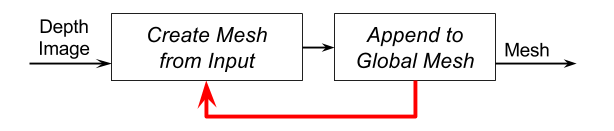
\includegraphics[width=.75\textwidth]{figures/diagram_general_pipeline.png}
  \caption{Common ``black box'' pipeline in black. The contribution of MABDI in red.}
  \label{fig:pipeline}
\end{figure}
